\documentclass[catalan, a4paper, nobib]{tufte-handout}

% encoding
\usepackage[utf8]{inputenc}
\usepackage[T1]{fontenc}
\usepackage{lmodern}
\usepackage{babel}

\frenchspacing
\usepackage[style=spanish]{csquotes}
\MakeAutoQuote{«}{»}

\usepackage{booktabs}
\usepackage{circuitikz}
\usepackage{siunitx}
\usepackage{amsmath}

\graphicspath{
    {fotos/}
}

% hyperlink setup / metadata
\usepackage{hyperref}
\AfterPreamble{\hypersetup{
  %%pdfauthor={},
  %%pdftitle={},
  %%pdfsubject={},
}}

% document metadata
\author{Víctor Méndez}
\title{ICOM: Pràctica 3}
\date{24-4-2024}

\begin{document}

\maketitle

\newthought{Activitat 3.1}

La potència més alta que pot ser representada és \qty[qualifier-mode=combine]{30}{\deci\bel\of{m}}. Hi ha \qty{10}{\deci\bel\per\text{div}}, per tant un ratio de \num{10}. Es representa entre \qty{0.982}{\giga\hertz} i \qty{1.018}{\giga\hertz}.

\begin{table}[h]
  \begin{center}
    \begin{tabular}{@{}cccc@{}}
      \toprule
      RBW & Span & Fs & Time \\
      \midrule
      \qty{172}{\kilo\hertz} & \qty{36}{\mega\hertz} & \qty{25}{\kilo\hertz} & \qty{22}{\micro\second} \\
      \bottomrule
    \end{tabular}
  \end{center}
\end{table}

\newthought{Activitat 3.2}

\begin{figure*}[!h]
  \begin{center}
    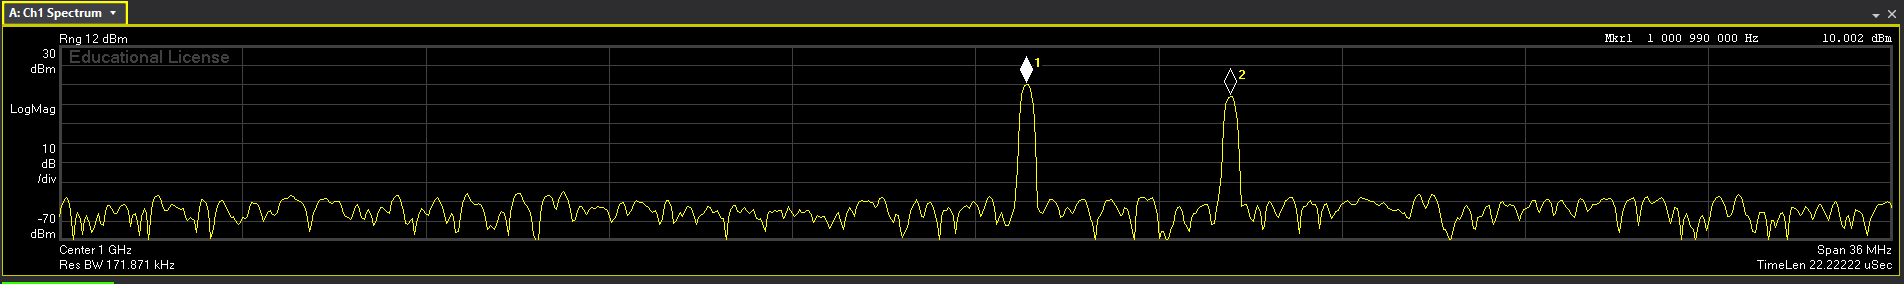
\includegraphics[width=465px]{q2_1.png}
  \end{center}
  \caption{Trace sencera}
\end{figure*}

Segons els marcadors, el primer sinusoide té una freqüència de \qty{1.0009}{\giga\hertz} i el segon \qty{1.0049}{\giga\hertz}. Les potencies son \qty[qualifier-mode=combine]{10}{\deci\bel\of{m}} i \qty[qualifier-mode=combine]{3.98}{\deci\bel\of{m}} respectivament. Les amplituds de les sinusoides son $\simeq\qty{1}{\volt}$ i $\simeq\qty{0.5}{\volt}$ respectivament. La resolució espectral val \qty{170}{\kilo\hertz} i la separació entre els components espectrals és de \qty{4}{\mega\hertz}; la resolució és més que suficient per distinguir aquests components.

\begin{figure}[!h]
  \begin{center}
    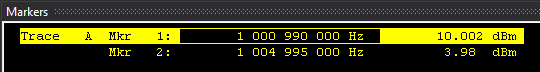
\includegraphics[width=300px]{q2_2.png}
  \end{center}
  \caption{Dades dels marcadors}
\end{figure}

\newthought{Activitat 3.3}

\begin{figure*}[!h]
  \begin{center}
    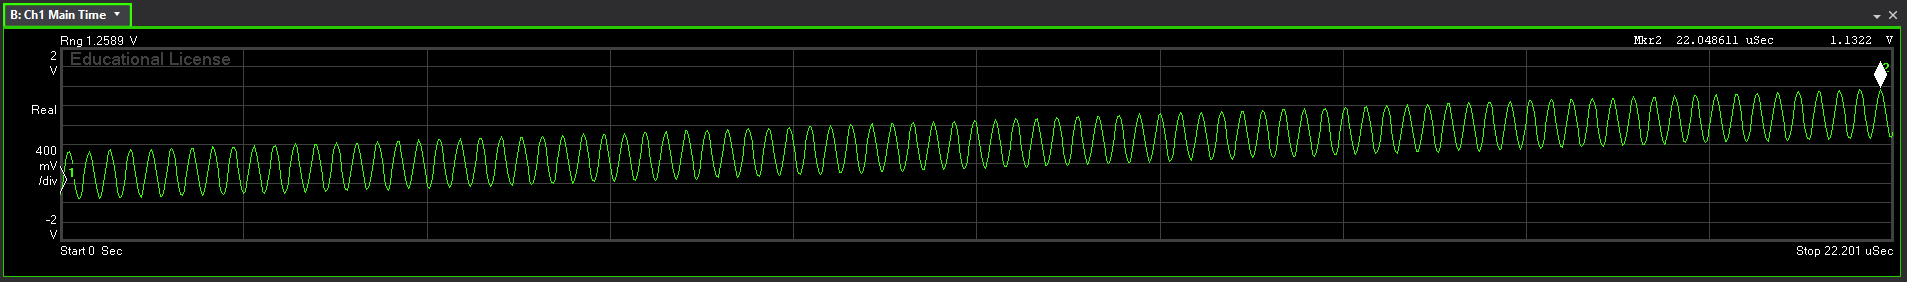
\includegraphics[width=465px]{q3_1.png}
  \end{center}
  \caption{Component en fase del senyal passabaix per $f_c=f_1=\qty{1.0009}{\giga\hertz}$}
\end{figure*}

Clarament la freqüència central triada per fer el senyal passabaix no és ben bé exacte. Com $f_c \ne f_1$ el que es veu és un cosinus de freqüència $\Delta f = f_c - f_1$ molt petita.

\newpage

En ajustar $f_c$ a \qty{1.001}{\giga\hertz} s'obtè el resultat teòric esperat; una constant sumada a un cosinus.

\begin{figure*}[!h]
  \begin{center}
    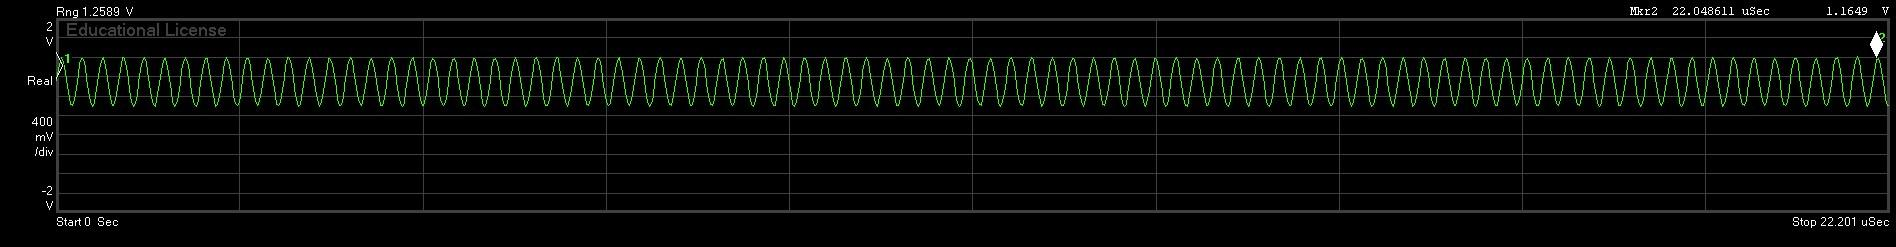
\includegraphics[width=465px]{q3_2.png}
  \end{center}
  \caption{Component en fase del senyal passabaix per $f_c=f_1=\qty{1.001}{\giga\hertz}$}
\end{figure*}

Si ajustem $f_c$ per a $f_2 = \qty{1.005}{\giga\hertz}$ s'obtè un resultant semblant.

\begin{figure*}[!h]
  \begin{center}
    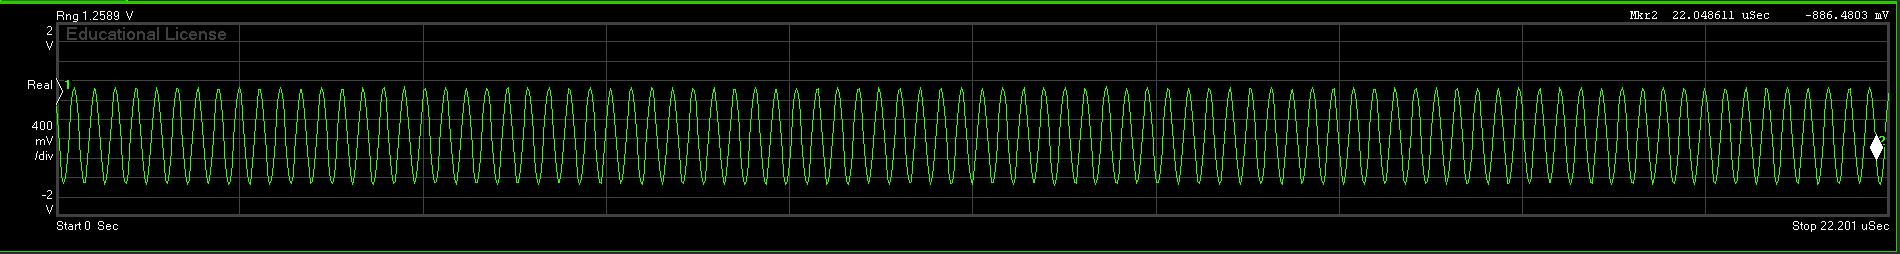
\includegraphics[width=465px]{q3_3.png}
  \end{center}
  \caption{Component en fase del senyal passabaix per $f_c=f_2=\qty{1.005}{\giga\hertz}$}
\end{figure*}

A partir d'aquestes dues imatges extreure la amplitud de cada component es trivial. Es mesura $A_1=\qty{0.98}{\volt}$ i $A_2=\qty{0.52}{\volt}$.

La mesura de les fases $\phi_1$ i $\phi_2$ és una mica més elaborada. A partir dels calculs teòrics es sap

\begin{align}
  f_c = f_1 \rightarrow i_s(t) &= A_1\cos{(\phi_1)} + A_2 \cos{(2\pi\,\Delta f\, t + \phi_2)} \\
  f_c = f_2 \rightarrow i_s(t) &= A_1\cos{(2\pi\,\Delta f\, t + \phi_1)} + A_2 \cos{(\phi_2)}
\end{align}

En altres paraules les components DC en cada cas depenen de una $A_i$ coneguda i una $\phi_i$ desconeguda.

Extreure el component DC no és dificil. Si per treure les amplituds fem servir $A_i=\frac{1}{2}\,\left[\text{max}(i_s)-\text{min}(i_s)\right]$, per obtenir el component DC farem ${DC}_i=\frac{1}{2}\,\left[\text{max}(i_s)+\text{min}(i_s)\right]$. Finalment

\begin{align}
  {DC}_i &= A_i \, \cos{(\phi_i)} \\
  \phi_i &= \arccos{\left(\frac{{DC}_i}{A_i}\right)}
\end{align}

Els resultats son $\phi_1=\ang{46.36}$ i $\phi_2=\ang{109.57}$. Els dos components tenen un desfasament de $\Delta\phi\simeq\ang{60}$.

\begin{figure}[!h]
  \begin{center}
    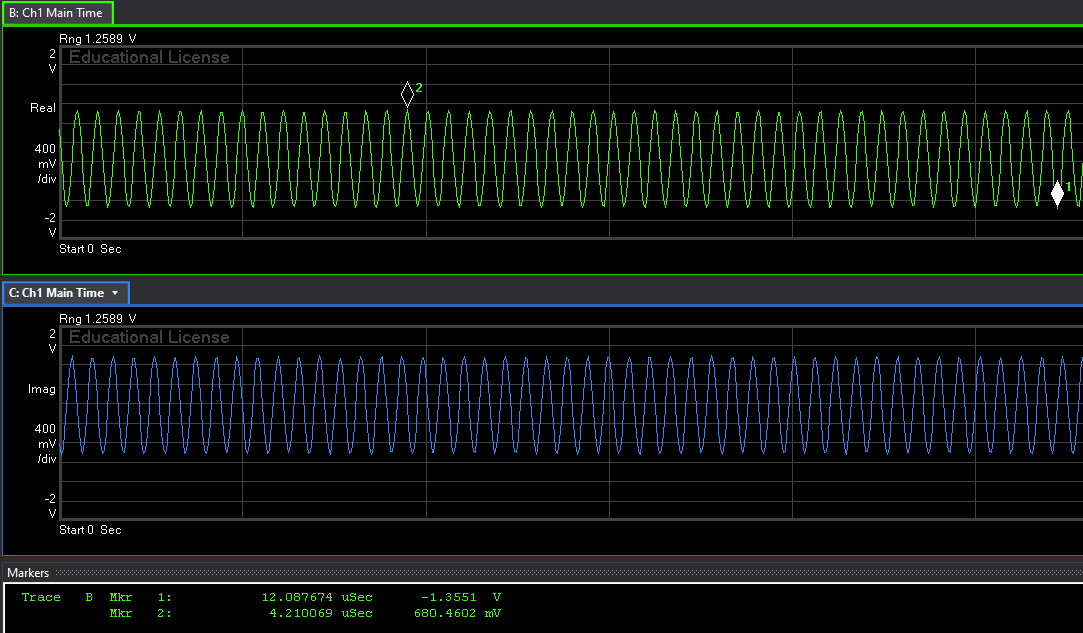
\includegraphics[width=205px]{q3_4.png}
  \end{center}
  \caption{Components en fase i quadratura}
\end{figure}

\end{document}